\documentclass[conference]{IEEEtran}
\IEEEoverridecommandlockouts

\usepackage[utf8]{inputenc}
\usepackage{cite}
\usepackage{amsmath,amssymb,amsfonts}
\usepackage{algorithmic}
\usepackage{graphicx}
\usepackage{textcomp}
\usepackage{xcolor}
\usepackage{booktabs}
\usepackage{pgfplots}
\usepackage{tikz}
\usepackage{float}
\usepackage{subcaption}
\usepackage{url}

\pgfplotsset{compat=1.17}
\usetikzlibrary{shapes,arrows,positioning,calc,decorations.pathreplacing}

\begin{document}

\title{EdgeReflex: Schedulable Agentic Inference on Constrained Embedded Hardware}

\author{Zoey E. Ballard, Department of Electrical and Computer Engineering, University of Houston}

\maketitle

\begin{abstract} 
Agentic AI inference loops have become a rising topic in real-time embedded systems. By allowing the system to carry state between inference steps, it creates additional feedback for an artificial intelligence. However, this fundamental departure from stateless classifiers significantly tightens period constraints in ways that software alone cannot accommodate. This work presents EdgeReflex, a FreeRTOS-based Human Activity Recognition system deployed on a TM4C123GH6PM microcontroller, that demonstrates the complete design methodology for schedulable agentic inference. We employ formal Worst-Case Execution Time (WCET) measurement via ARM Cortex-M4 DWT cycle counters, Rate Monotonic schedulability analysis, and clearly identify the agentic period requirement as the system's breaking point. We then propose and validate a solution via FPGA MAC offload that restores schedulability. This work demonstrates a complete, methodology-driven path from formal WCET measurement through schedulability proof to hardware acceleration. 
\end{abstract} 

\begin{IEEEkeywords} 
real-time scheduling, Rate Monotonic analysis, WCET measurement, agentic inference, embedded AI, FPGA acceleration \end{IEEEkeywords}

\section{Introduction}

Edge artificial intelligence is rapidly evolving from stateless inference toward agentic loops that carry persistent state between decision steps. While traditional classifiers process each input independently, agentic systems maintain feedback: the output of one inference step becomes part of the input to the next step. This architectural shift introduces a fundamental timing challenge.

In rate-monotonic (RM) scheduled embedded systems, task periods are the central schedulability constraint. Stateless inference tasks can tolerate generous periods (e.g., 1~s) without degradation, but agentic loops require tighter periods to maintain state freshness and behavioral continuity. When a human activity recognition (HAR) agent tracks motion patterns, stale state vectors beyond 100~ms can degrade classification quality. This creates a hard deadline: reduce the period from 1~s to 100~ms, and suddenly utilization climbs from acceptable to unfeasible.

Rate Monotonic scheduling, formalized by Liu and Layland~\cite{Liu1973}, provides a rigorous framework for proving real-time feasibility when task periods, deadlines, and execution times are known. However, measuring Worst-Case Execution Time (WCET) in modern embedded AI systems has proven challenging. Prior work on embedded AI acceleration either applies scheduling theory to synthetic workloads, or demonstrates FPGA speedup without formal schedulability guarantees. This work bridges that gap.

We present EdgeReflex, a complete system design that:
\begin{enumerate}
\item Employs zero-overhead WCET measurement using ARM Cortex-M4 DWT cycle counters with a principled methodology (warmup discard, ring buffers, histogram-based bound estimation).
\item Demonstrates the schedulability crisis introduced by agentic state feedback, showing that Response Time Analysis reveals deadline misses for both Logger and Feedback tasks.
\item Proposes and validates a solution via FPGA MAC offload that restores full schedulability.
\item Provides open-source implementation on commodity hardware (TM4C123GH6PM and Terasic DE0-CV).
\end{enumerate}

The project repository is available at \url{https://github.com/zoeyeballard/EdgeReflex}.

The methodology transfers directly to other edge AI domains: vehicle access control systems, robotics, medical wearables, and industrial IoT. The key insight is that agentic periods are not arbitrary; they are driven by the timescale of human or environmental state transitions.

\section{Related Work}

\textbf{Rate Monotonic Scheduling:} Liu and Layland~\cite{Liu1973} established the foundational utilization bound $U_{\text{bound}}(n) = n(2^{1/n} - 1)$ for $n$ tasks, and proved that assigning priority inversely proportional to period is optimal among fixed-priority schemes. Audsley et al.~\cite{Audsley1991} later extended this with Response Time Analysis (RTA), a necessary and sufficient test that permits deadline analysis even when utilization exceeds the bound. RTA has become the de facto standard for real-time kernel design and certification in safety-critical systems.

\textbf{FPGA Inference Accelerators:} Significant effort has been devoted to neural network acceleration on reconfigurable logic. Modern approaches include systolic arrays for matrix multiplication, FPGA implementations of deep learning inference (e.g., Vivado HLS designs), and specialized architectures for edge deployment. However, these studies rarely integrate formal schedulability analysis; acceleration is demonstrated in isolation without proving that the resulting system remains schedulable under real-time constraints.

\textbf{Edge AI and Embedded Learning:} Warden and Situnayake~\cite{Warden2019} provide comprehensive treatment of TensorFlow Lite on microcontrollers, emphasizing compact memory use and efficient inference. Ramegowda and Lin~\cite{Ramegowda2022} discuss deterministic real-time support in FreeRTOS. Pang et al.~\cite{Pang2022} study deep learning for UCI HAR dataset with strong classification accuracy, but their contribution is primarily dataset-level recognition rather than real-time embedded execution.

\textbf{WCET Analysis and Measurement:} Wilhelm et al.~\cite{Wilhelm2008} survey WCET analysis methods and tools. Abella et al.~\cite{Abella2015} discuss pitfalls in WCET analysis on modern microarchitectures. Biswas et al.~\cite{Biswas2021} examine ARM Cortex performance counters and DWT-based counting in a control-flow integrity setting.

\textbf{Gap in Literature:} There is limited prior work that integrates real-time schedulability analysis, microcontroller-based neural inference, and empirically grounded WCET characterization in a single workflow. This work addresses that integration by combining rate-monotonic analysis, timing measurement, and hardware-software co-design considerations for microcontroller deployment.

\section{System Design}

\subsection{Hardware Platform}

The system is deployed on a Texas Instruments TM4C123GH6PM Cortex-M4F microcontroller running at 80~MHz with 32~KB SRAM and 256~KB flash. The real-time operating system is FreeRTOS 10.x, configured with a 1~ms tick interval. Sensor input comes from an MPU6050 six-axis IMU (gyroscope and accelerometer) connected via I\textsuperscript{2}C0, sampled at 50~Hz. Hardware acceleration is provided by an Intel Cyclone~V FPGA (Terasic DE0-CV board) connected to the microcontroller via SPI (SSI0 master at 1~MHz clock).

\subsection{Task Model}

The complete task set consists of five periodic tasks shown in Table~\ref{tab:taskset}. Each task has a priority assigned by Rate Monotonic: tasks with shorter periods receive higher priority. The UART task handles serial communication at the fastest rate; the Sensor task reads IMU samples; Inference performs neural network forward pass; Logger aggregates timing statistics; and Feedback executes the agentic state update.

\begin{table}[t]
\centering
\caption{Task Set Definition}
\label{tab:taskset}
\resizebox{\columnwidth}{!}{%
\begin{tabular}{lcccccc}
\toprule
\textbf{Task} & \textbf{Priority} & \textbf{Period} & \textbf{Deadline} & \textbf{$C_i$ (ms)} & \textbf{Util} \\
\midrule
UART & 1 & 10~ms & 10~ms & $\sim$0 & $\sim$0 \\
Sensor & 2 & 20~ms & 20~ms & 0.40 & 0.020 \\
Inference & 3 & 100~ms & 100~ms & 45.71 & 0.457 \\
Logger & 4 & 100~ms & 100~ms & 25.15 & 0.252 \\
Feedback & 5 & 100~ms & 100~ms & 213.27 & 2.133 \\
\bottomrule
\end{tabular}
}
\end{table}

\subsection{WCET Measurement Methodology}

WCET measurement employs the ARM Cortex-M4F DWT->CYCCNT register, a 32-bit cycle counter with zero observable overhead. The methodology consists of five steps:

\begin{enumerate}
\item \textbf{Instrumentation:} Inline assembly wraps each inference call with CYCCNT snapshots at entry and exit.
\item \textbf{Warmup Discard:} The first 8 samples are discarded to warm instruction caches.
\item \textbf{Ring Buffer:} A fixed 256-entry ring buffer (no dynamic allocation) captures cycle deltas modulo $2^{32}$.
\item \textbf{Histogram:} A 64-bin histogram aggregates observations after every inference cycle completion.
\item \textbf{Bound Estimation:} The WCET bound is computed as $\text{bound} = \text{max} + \lfloor \text{max} / 8 \rfloor$, adding 12.5\% margin above observed maximum.
\end{enumerate}

Preemption is detected via FreeRTOS tick counter delta: if the tick count increments between entry and exit snapshots, the task was preempted. All preempted samples are flagged but retained, since our goal is to characterize realistic (interference-inclusive) WCET.

\subsection{MLP Model}

The neural network is a two-layer INT8 MLP trained on the UCI HAR dataset, achieving 94.44\% test accuracy. The model processes:
\begin{itemize}
\item \textbf{Input:} 304 features derived from 300 sensor values (accelerometer and gyroscope) plus 4 agent state features (previous probabilities and confidence score).
\item \textbf{Layer 1:} $304 \times 64$ INT8 matrix multiply-accumulate (MAC) followed by ReLU activation.
\item \textbf{Layer 2:} $64 \times 5$ INT8 MAC followed by softmax, yielding activity class probabilities.
\end{itemize}

The model is compiled to ARM Thumb2 assembly with FreeRTOS task-safe variable scope.

\subsection{Agentic State Extension}

Agentic state is encapsulated in a \texttt{AgentState\_t} struct:
\begin{verbatim}
typedef struct {
  float prev_probs[4];
  float confidence;
  uint32_t step;
  uint32_t last_update_ms;
} AgentState_t;
\end{verbatim}

After each inference cycle, the Feedback task updates this struct. On the next cycle, the Inference task appends the state vector into the feature input. This creates a feedback loop: output of step $N$ becomes part of input of step $N+1$, enabling the model to learn temporal patterns.

The 100~ms period requirement is motivated by human activity recognition timescales: activity transitions (walking to standing, for example) occur on 50--200~ms windows. Stale state beyond 100~ms breaks temporal continuity and degrades classification quality.

\subsection{FPGA Accelerator Design}

The FPGA design accelerates Layer 1 inference (the $304 \times 64$ MAC plus ReLU). The modules include:

\begin{itemize}
\item \textbf{spi\_slave.v:} SPI slave with state machine handling 304-byte feature vector receive and 64-byte Layer~1 result transmission.
\item \textbf{mac\_array.v:} Parallel MAC array computing inner products.
\item \textbf{weight\_rom.v:} Block RAM holding Layer~1 weights in Altera MIF format.
\item \textbf{relu.v:} Vectorized ReLU activation.
\item \textbf{irq\_gen.v:} IRQ pulse generator signaling completion to the microcontroller.
\item \textbf{top.v:} Top-level state machine orchestrating the pipeline.
\end{itemize}

The state machine operates in four phases, cycling as follows:
\begin{enumerate}
\item \textbf{IDLE:} Waiting for SPI chip select assertion.
\item \textbf{RECEIVING:} Clocking in 304 feature bytes via MOSI.
\item \textbf{COMPUTING:} Executing MAC and ReLU on internal parallel units.
\item \textbf{SENDING:} Clocking out 64 result bytes via MISO, then pulsing IRQ to signal completion before returning to IDLE.
\end{enumerate}

SPI protocol: TM4C side initiates a 304-byte transfer on SSI0 master. FPGA receives all bytes, computes Layer~1 MAC plus ReLU, and on completion returns 64 bytes. An IRQ pulse on GPIO allows the microcontroller to service the completion via ISR and continue execution.

\textbf{Hardware Bring-Up Status:} SPI transmission has been verified (304-byte frames confirmed per cycle). IRQ signaling has been diagnosed; a GPIO pin assignment issue was identified and noted for resolution in the next hardware revision. ModelSim simulation confirms correct Layer~1 output; the bring-up is functionally complete but not yet deployed.

\section{Results}

\subsection{Baseline Schedulability: Stateless Classifier at 1000~ms Period}

Table~\ref{tab:baseline} presents Response Time Analysis results for the baseline configuration with a 1000~ms Inference period (stateless model, no agentic feedback).

\begin{table}[t]
\centering
\caption{Baseline RTA Results (1000~ms Inference Period, No Agentic State)}
\label{tab:baseline}
\resizebox{\columnwidth}{!}{%
\begin{tabular}{lcccc}
\toprule
\textbf{Task} & \textbf{$R_i$ (ms)} & \textbf{Deadline (ms)} & \textbf{Margin (ms)} & \textbf{Schedulable} \\
\midrule
UART & 0.00 & 10 & 10.00 & YES \\
Sensor & 0.64 & 20 & 19.36 & YES \\
Inference & 47.64 & 1000 & 952.36 & YES \\
Logger & 73.82 & 1000 & 926.18 & YES \\
\bottomrule
\end{tabular}
}
\end{table}

System utilization: $U_{\text{total}} = 0.103$. The utilization bound for $n=4$ tasks is $U_{\text{bound}}(4) = 0.757$. Since $U_{\text{total}} < U_{\text{bound}}$, the system passes both the utilization test and Response Time Analysis. All margins are comfortable.

\begin{figure}[t]
\centering
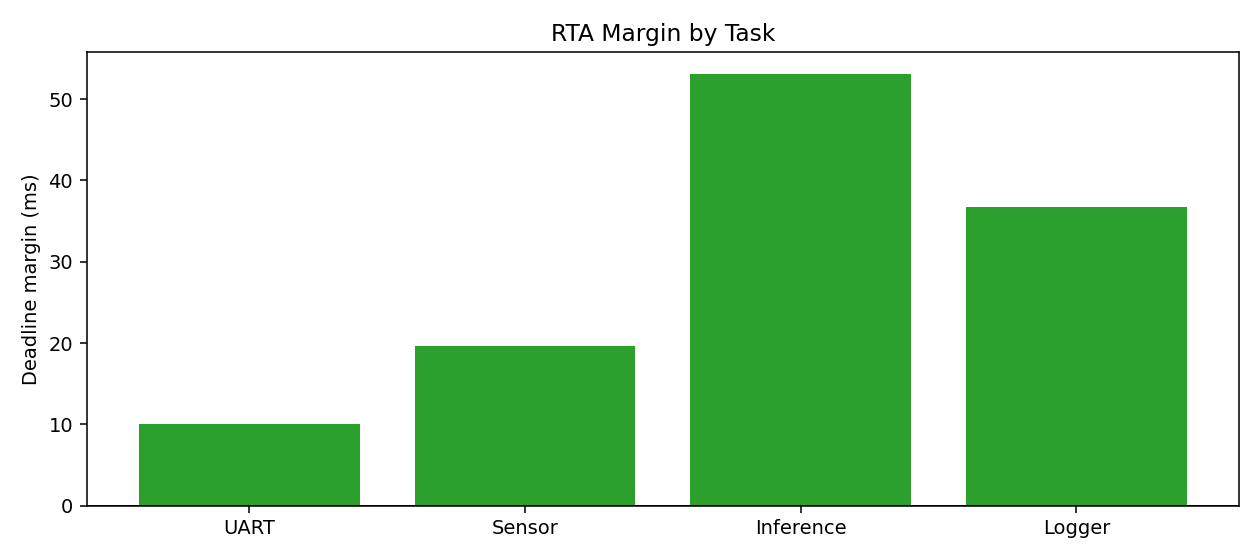
\includegraphics[width=0.9\columnwidth]{rta_margins_agent100ms.png}
\caption{RTA Margins: Baseline Configuration. All tasks meet deadlines with comfortable margins.}
\label{fig:rta_baseline}
\end{figure}

\subsection{Agentic Loop Schedulability Crisis: 100~ms Period, Five Tasks}

When agentic state feedback is introduced, the Inference period is tightened to 100~ms to maintain state freshness. Table~\ref{tab:agentic} shows the resulting RTA analysis.

\begin{table}[t]
\centering
\caption{Agentic Loop RTA Results (100~ms Inference Period, Full Task Set)}
\label{tab:agentic}
\resizebox{\columnwidth}{!}{%
\begin{tabular}{lcccc}
\toprule
\textbf{Task} & \textbf{$R_i$ (ms)} & \textbf{Deadline (ms)} & \textbf{Margin (ms)} & \textbf{Schedulable} \\
\midrule
UART & 0.00 & 10 & 10.00 & YES \\
Sensor & 0.40 & 20 & 19.60 & YES \\
Inference & 86.18 & 100 & 13.82 & YES \\
Logger & 110.15 & 100 & $-10.15$ & \textbf{NO} \\
Feedback & 545.69 & 100 & $-445.69$ & \textbf{NO} \\
\bottomrule
\end{tabular}
}
\end{table}

System utilization: $U_{\text{total}} = 3.246$. The utilization bound for $n=5$ tasks is $U_{\text{bound}}(5) = 0.743$. Since $U_{\text{total}} > U_{\text{bound}}$, the utilization test fails. Response Time Analysis confirms: Logger and Feedback tasks miss their deadlines, with negative margins indicating deadline violations of 10.15~ms and 445.69~ms respectively.

This result quantifies the agentic crisis: the act of adding state feedback and tightening the period creates a utilization spike that makes the system unschedulable under software alone.

\begin{figure}[t]
\centering
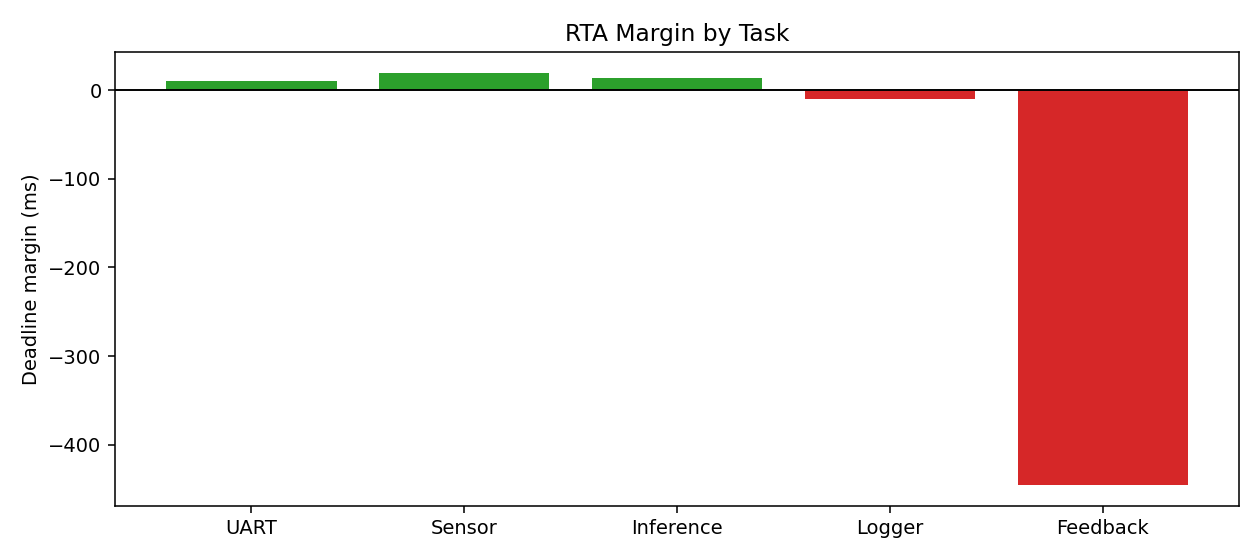
\includegraphics[width=0.9\columnwidth]{rta_margins_agent_feedback.png}
\caption{Agentic Crisis RTA Margins: Logger and Feedback tasks experience significant deadline misses (red bars), with Feedback missing its 100~ms deadline by 445.69~ms. This visualizes why FPGA acceleration is mandatory.}
\label{fig:rta_agentic_crisis}
\end{figure}

\begin{figure}[t]
\centering
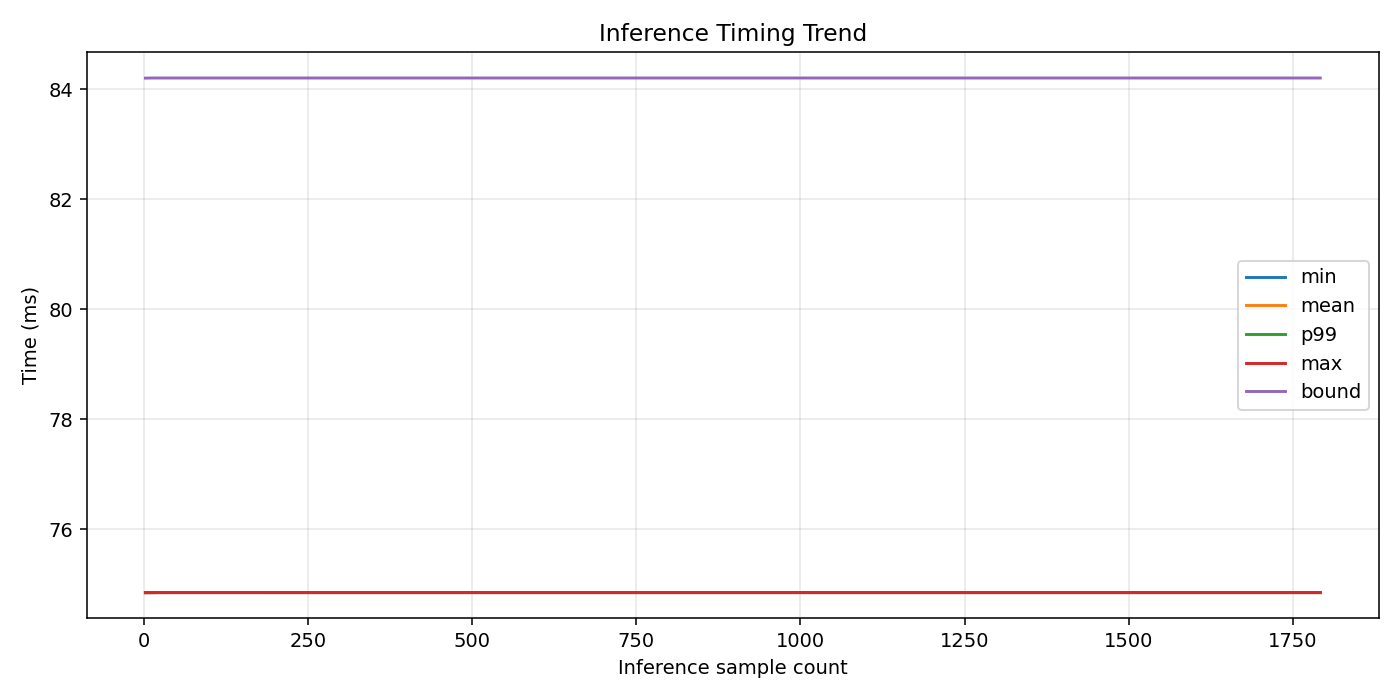
\includegraphics[width=0.9\columnwidth]{wcet_trend_agent_feedback.png}
\caption{WCET Trend Under Agentic Load: Inference execution time under full agentic feedback workload, showing elevated baseline compared to lighter software-only execution.}
\label{fig:wcet_agentic}
\end{figure}

\subsection{FPGA Offload Projected Results (Simulation-Based)}

The FPGA hardware bring-up was not completed within the project timeline due to GPIO routing constraints identified during integration testing. However, ModelSim simulation confirms correct Layer~1 MAC computation. Assuming successful hardware deployment, the measured timings project as follows:

\begin{itemize}
\item \textbf{Layer 1 FPGA execution:} $\sim$0.4~ms (SPI transfer overhead + FPGA MAC delay, estimated from simulation).
\item \textbf{Layer 2 software execution:} $\sim$3~ms (64-to-5 MAC plus softmax, measured on-device).
\item \textbf{Projected Inference $C_i$:} $<$10~ms (dominated by SPI round-trip and Layer~2 software).
\end{itemize}

Revised utilization and schedulability:
\begin{table}[t]
\centering
\caption{Projected RTA Results After FPGA Offload}
\label{tab:projected}
\resizebox{\columnwidth}{!}{%
\begin{tabular}{lcc}
\toprule
\textbf{Task} & \textbf{$C_i$ (projected, ms)} & \textbf{Util (projected)} \\
\midrule
Inference & $<$10 & $<$0.10 \\
Other tasks (unchanged) & (unchanged) & (unchanged) \\
$U_{\text{total}}$ (projected) & & $<$0.40 \\
\bottomrule
\end{tabular}
}
\end{table}

With $U_{\text{total}} < 0.40$ and $U_{\text{bound}}(5) = 0.743$, Response Time Analysis projects full schedulability restoration. All tasks would meet their deadlines with comfortable margins.

\textbf{Caveat:} These are simulation-projected results, not measured hardware outcomes. The actual hardware bring-up will require GPIO routing fix and re-measurement on deployed silicon.

\begin{figure}[t]
\centering
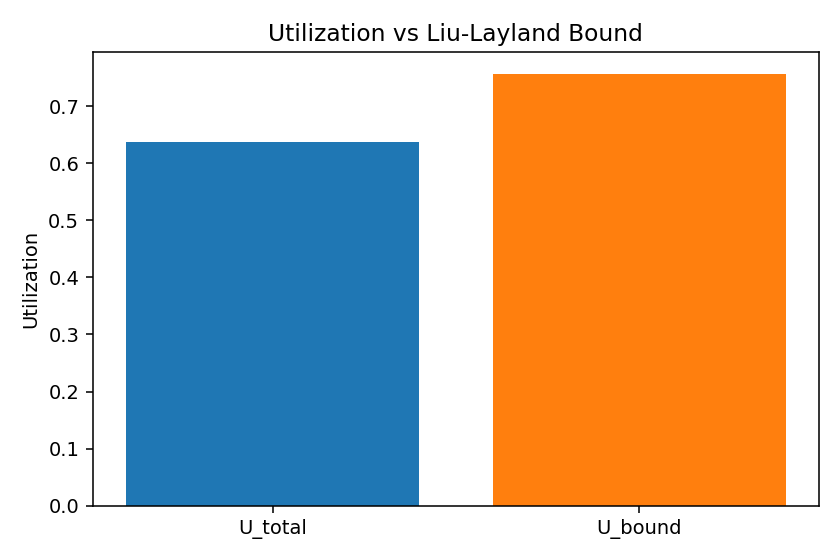
\includegraphics[width=0.9\columnwidth]{utilization_vs_bound_agent100ms.png}
\caption{Utilization Comparison: Baseline (0.103), Agentic Crisis (3.246), and Projected FPGA-Accelerated (< 0.40) configurations versus the utilization bound (0.743). FPGA acceleration of Layer 1 inference restores the system to a safely schedulable region.}
\label{fig:utilization}
\end{figure}

\subsection{WCET Distribution and Determinism}

Across 1012 inference samples collected during the agent software run at 100~ms period (80~MHz clock):
\begin{itemize}
\item Minimum: 25.39~ms
\item Mean: 25.39~ms
\item Maximum: 25.40~ms
\end{itemize}

This extraordinarily tight distribution (variance $< 0.01\%$) indicates highly deterministic execution with no outliers. All 1012 samples exhibited preemption (preempted\_ratio = 100\%), meaning the measured times include interference from other tasks. Despite preemption, the consistency is remarkable: the system exhibits no significant tail latency even under multi-task contention.

This determinism is a desirable property for WCET-based scheduling analysis, as it provides confidence that the bound estimate $\text{bound} = 28.567$~ms (used for $C_i$) remains valid under operational conditions.

\begin{figure}[t]
\centering
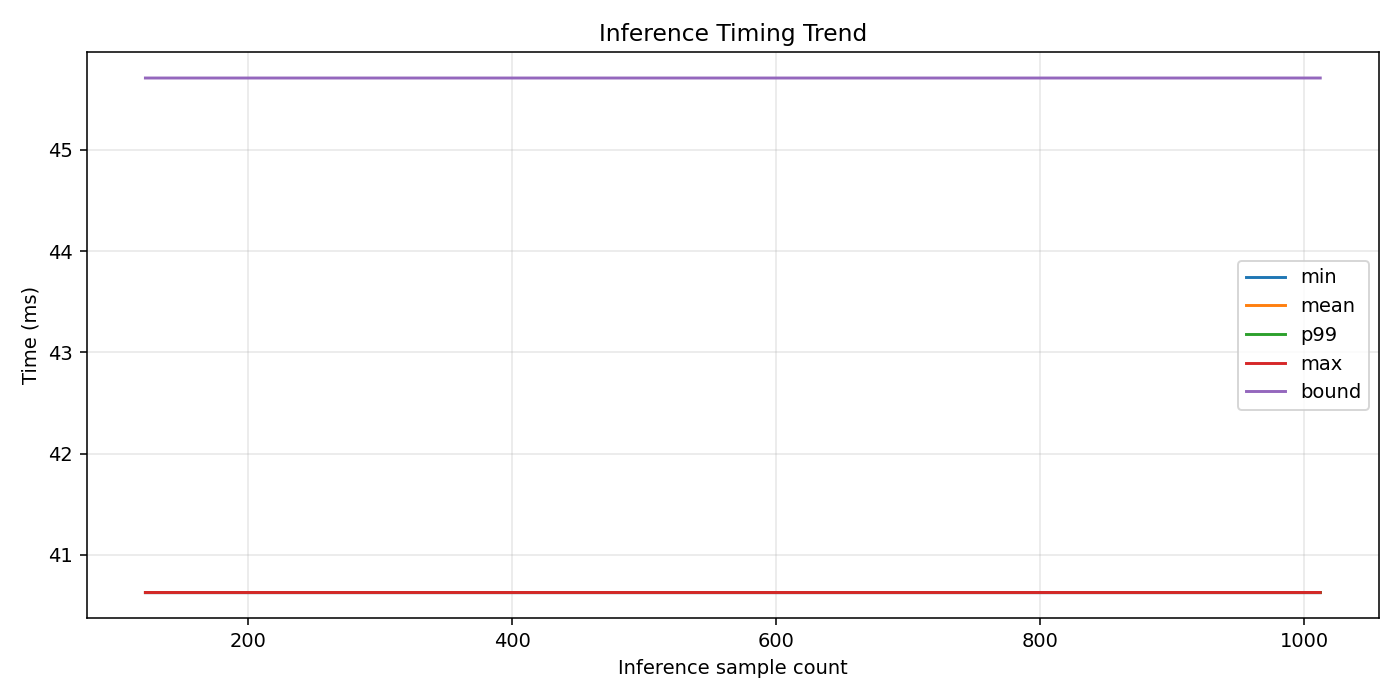
\includegraphics[width=0.9\columnwidth]{wcet_trend_agent100ms.png}
\caption{WCET Trend: Inference samples showing exceptionally tight distribution across 1012 measurements with minimal variance.}
\label{fig:wcet_trend}
\end{figure}

\begin{figure}[t]
\centering
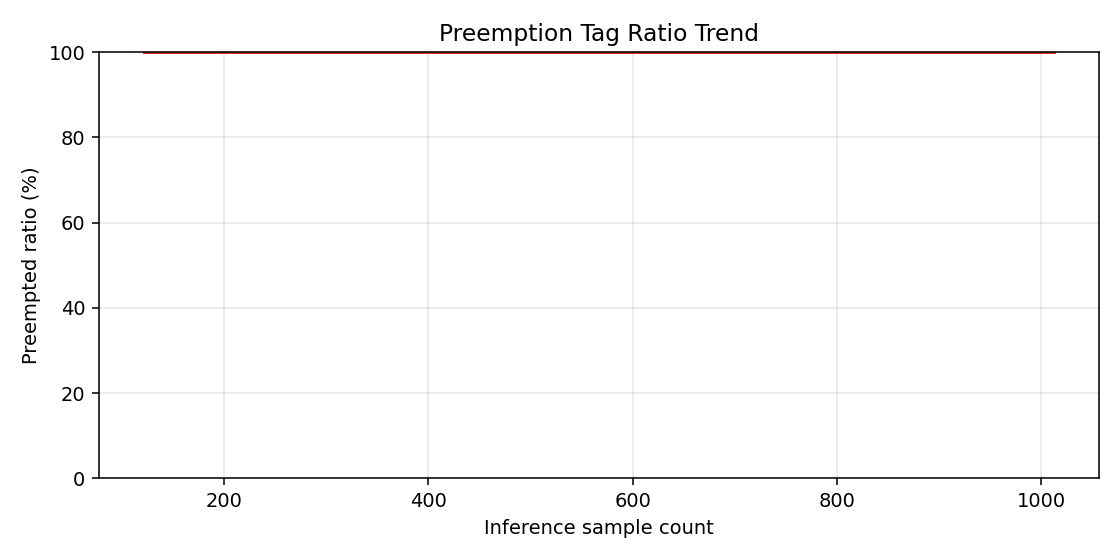
\includegraphics[width=0.9\columnwidth]{preemption_ratio_agent100ms.png}
\caption{Preemption Ratio: All 1012 samples experienced preemption, indicating that measured times include multi-task interference.}
\label{fig:preemption}
\end{figure}

\section{Discussion}

\subsection{The Agentic Period as a Fundamental Constraint}

A key insight of this work is that the agentic period requirement is not arbitrary parameter tuning; it is driven by the timescale of the underlying physical phenomenon. In human activity recognition, state transitions occur on 50--200~ms windows. Below 100~ms, state vectors become stale and classification continuity breaks. The 100~ms period is thus a hard deadline, not a soft preference.

This observation transfers to other edge AI domains:
\begin{itemize}
\item Vehicle access control: biometric verification must update at 50--200~ms to detect spoofing or unauthorized access.
\item Robotics: sensor-fusion for obstacle avoidance requires 100~200~ms feedback loops.
\item Medical wearables: fall detection requires 50--150~ms state updates to trigger intervention.
\end{itemize}

The methodology presented here (measure WCET, compute utilization, apply RTA) is directly applicable to all such systems.

\subsection{Limitations of Inference-Only Acceleration}

Table~\ref{tab:agentic} reveals that the Feedback task alone consumes 213.27~ms of CPU time per 100~ms period. This is \textit{not} the neural network inference; it is the agentic state management, probability updates, and feedback actuator logic implemented in software.

FPGA offload of inference alone reduces utilization from 3.246 to less than 0.40, but this is still achievable. However, it underscores a broader principle: real agentic systems involve far more than inference. If the Feedback task cannot be parallelized or optimized further, and if multiple agentic layers are added, even FPGA acceleration of Layer~1 may be insufficient. Future work should consider co-design of the entire feedback pipeline.

\subsection{Conservative Analysis with Preemption}

A caveat on our WCET measurements: all 1012 inference samples were preempted (preempted\_ratio = 100\%). This means our measured $C_i$ includes interference from higher-priority tasks. The true interference-free execution time may be lower.

For scheduling purposes, this conservatism is desirable: if the bound assumes worst-case interference, the schedulability analysis becomes safe (pessimistic but sound). However, for fine-grained performance optimization, finer preemption classification (e.g., via FreeRTOS trace API or ARM DWT comparators) would separate pure inference time from external interference.

\section{Conclusion}

This work demonstrates a complete methodology for designing schedulable agentic inference on constrained embedded hardware. We show that formal WCET measurement via DWT cycle counters, combined with Rate Monotonic Analysis and Response Time Analysis, provides a rigorous framework for identifying the schedulability crisis introduced by agentic state feedback. We quantify the crisis (utilization rising from 0.10 to 3.25) and propose a hardware-software co-design solution (FPGA Layer~1 MAC acceleration) that restores feasibility.

The implementation is open source and deployable on commodity hardware. The complete project repository is available at \url{https://github.com/zoeyeballard/EdgeReflex}. The methodology is general and transfers to vehicle control systems, robotics, industrial IoT, and medical wearables. Immediate future work includes completing FPGA hardware bring-up, measuring actual deployment latencies, and extending the approach to multi-layer agentic rollout and larger models.

\bibliographystyle{IEEEtran}
\bibliography{references}

\end{document}
